\documentclass[../main.tex]{subfiles}
% !TeX root = ../main.tex
\begin{document}
	\section{Completing the Accounting Cycle}
	
	An \textbf{unadjusted trial balance} is a list of accounts and balances 
	prepared 
	before adjustments are recorded. An \textbf{adjusted trial balance} is a 
	list of 
	accounts and balances prepared after adjusting entries have been recorded 
	and posted to the ledger.
	
	\begin{figure}[ht]
		\centering
		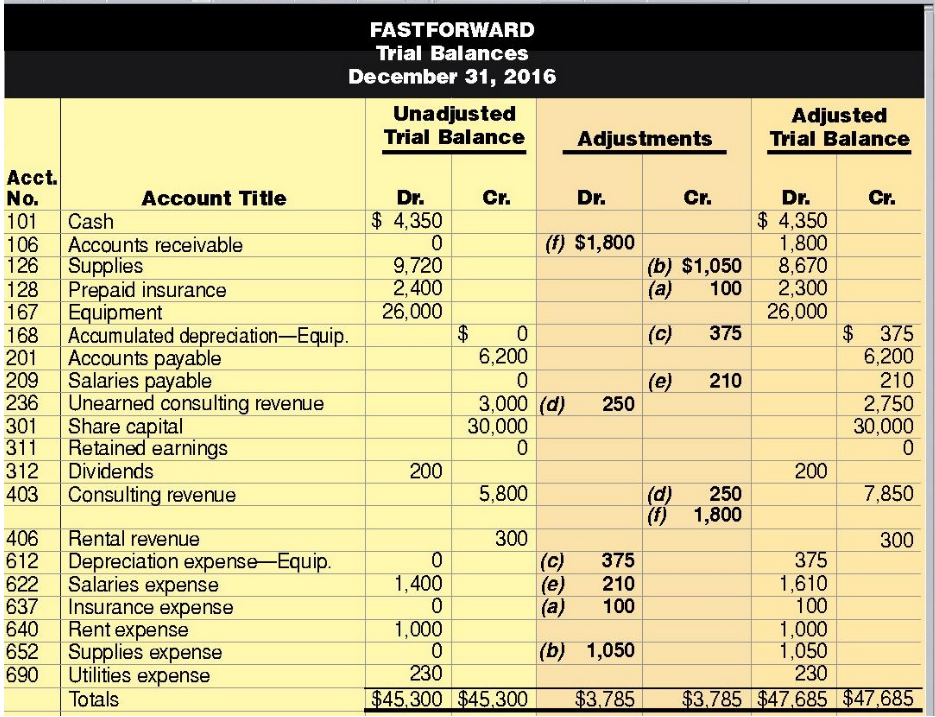
\includegraphics[width=1\columnwidth]{images/c4/trial_balance_adjusted.png}
		\caption{\textbf{Unadjusted and Adjusted Trial Balance.} Several new 
		accounts arise from the adjusting entries. Each adjustment (see middle 
		columns) is identified by a letter in parentheses that links it to an 
		adjusting entry explained earlier. Each amount in the Adjusted Trial 
		Balance columns is computed by taking that account’s amount from the 
		Unadjusted Trial Balance columns and adding or subtracting any 
		adjustment}
	\end{figure}
	
	A \textbf{work sheet} is not a required report but it has the following 
	benefits:
	\begin{itemize}[noitemsep]
		\item aids the preparation of financial statements.
		\item reduces the possibility of errors.
		\item links accounts and adjustments
		\item assists in planning and organizing an audit 
		\item helps in preparing interim financial statements
		\item shows the effects of proposed transactions.
	\end{itemize}
	
	
	\subsection{Preparing Financial Statements}
	
	The adjusted trial balance is used to prepare the company's financial 
	statements. The followings steps are taken:
	\begin{enumerate}[noitemsep]
		\item Prepare the income statement
		\begin{figure}[ht]
			\centering
			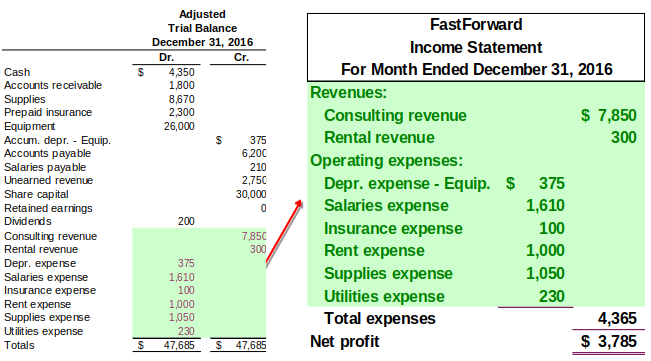
\includegraphics[width=\columnwidth]{images/c4/preparing_income_statement.png}
			\caption{Preparing the Income Statement}
		\end{figure}
		\item Prepare the statement of changes in equity - net profit from 
		Income Statement:
		\begin{figure}[ht!]
			\centering
			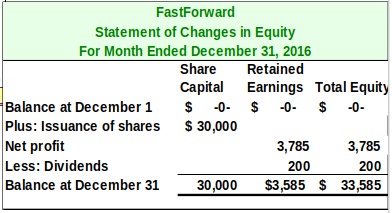
\includegraphics[width=0.8\columnwidth]{images/c4/statement_of_sce.png}
			\caption{Preparing the Income Statement}
		\end{figure}
		\item Prepare the statement of financial position - Asset and 
		liability balances are transferred over from the adjusted trial balance 
		to the Statement of Financial Position. The ending equity balance was 
		determined on the Statement of Changes. The ending balance is 
		transferred from that statement to the Statement of Financial Position. 
		
		\begin{figure}[ht!]
			\centering
			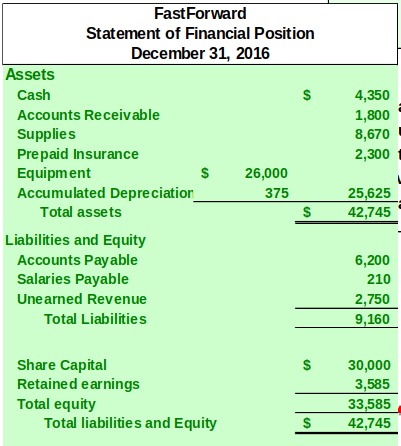
\includegraphics[width=0.80\columnwidth]{images/c4/statement_of_financial_position.png}
			\caption{Preparing the Statement of Financial Position}
		\end{figure}
		
	\end{enumerate}

	\subsection{Classified Statement of Financial Position}
	
	A classified statement of financial position is the most popular format 
	used by business. On the asset side of the statement of financial position 
	we group assets as current or noncurrent. 
	
	\begin{figure}[ht!]
		\centering
		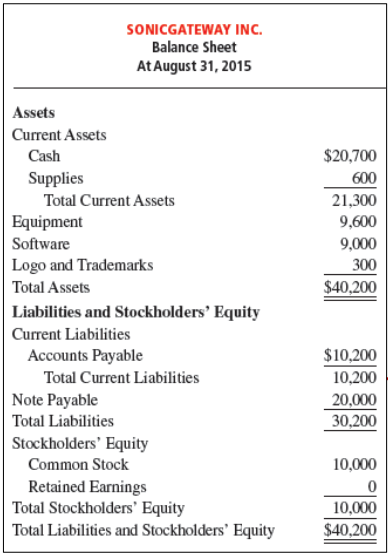
\includegraphics[width=0.70\columnwidth]{images/c4/classified_balance_sheet.png}
		\caption{Classified Balance Sheet}
	\end{figure}

	The classified balance sheet format makes it easy to see whether current 
	assets are sufficient to pay current liabilities \eg current ratio. 
	
	A \textbf{current asset} is one that is 
	expected to be converted into cash in one year or the company’s normal 
	operating cycle, whichever is longer. The operating cycle of a company is 
	the time it takes to acquire inventory, sell the inventory, and collect 
	cash. For many companies the operating is less than one year. These 
	companies would classify an asset as current as long as that asset is 
	expected to be converted into cash within one year.
	
	On the liabilities plus equity side of the statement of financial position, 
	we divide liabilities between current and noncurrent. A \textbf{current 
	liability} 
	is one we expect to be paid out of the company’s current assets within the 
	longer of one year or the normal operating cycle.
	
	Current or short-term items are those expected to come due \ie 
	collected/owed within the longer of one year or the company's normal 
	operating cycle, whichever is longer.
	
	\subsubsection{Current Assets}
	
	Current assets are expected ot be sold, collected, or used within one year 
	or the company's operating cycle, whichever is longer. Current assets 
	normally include cash, short-term investments, accounts receivable, 
	merchandise inventory, office supplies, and prepaid expenses.
	
	Short-term investments are expected to be sold within one year or the 
	normal operating cycle, whichever is longer.
	
	Merchandise inventory contains inventory items we expect to sell to 
	customers in the normal course of business. For a service business, we 
	would not expect to find a merchandise inventory account. 
	
	\subsubsection{Noncurrent Assets}
	
	Noncurrent assets are not used up within one year or the operating cycle, 
	whichever is longer. 
	
	They generally include long-term financial assets which are likely to be 
	investments in other entities’ shares or bonds. Property, plant and 
	equipment (PPE) are tangible assets that are both long-term and used to 
	produce or sell products and services.
	
	Intangible assets are long-term resources that benefit business operations, 
	usually lack physical form, and have uncertain benefits. Their value comes 
	from the privileges or rights granted to or held by the owner \eg 
	intellectual property. 
	
	\subsubsection{Current Liabilities}
	
	Current liabilities are obligations due within one year or the company's 
	operating cycle, whichever is longer. Current liabilities normally include 
	accounts payable, wages payable, 
	short-term notes payable, and the current portion of long-term liabilities. 
	
	\subsubsection{Noncurrent Liabilities}
	
	Noncurrent Liabilities are obligations not due within one year or the 
	company's operating cycle, whichever is longer. 
	
	\subsubsection{Equity}
	
	The equity section of the classified statement of financial position 
	includes the updated retained earnings account.
	
	\subsection{The Accounting Cycle}
	The term accounting cycle refers to the steps in preparing financial 
	statements. It is called a cycle because the steps are repeated each 
	reporting period. There are ten steps in the cycle which include:
	\begin{enumerate}[noitemsep]
		\item \textbf{Analyze transactions} - Analyze transactions to prepare 
		for 
		journalizing.
		\item \textbf{Journalize} - Record accounts, including debits and 
		credits, in a journal.
		\item \textbf{Post} - Transfer debits and credits from the journal to 
		the ledger.
		\item \textbf{Prepare unadjusted trial balance} - Summarize unadjusted 
		ledger accounts and amounts.
		\item \textbf{Adjust} - Record adjustments to bring account balances 
		up to date; journalize and post adjustments
		\item \textbf{Prepare adjusted trial balance} - Summarize adjusted 
		ledger accounts and amounts.
		\item \textbf{Prepare statements} - Use adjusted trial balance to 
		prepare financial statements.
		\item \textbf{Close} - Journalize and post entries to close temporary 
		accounts.
		\item \textbf{Prepare post-closing trial balance} - Test clerical 
		accuracy of the closing procedures.
		\item \textbf{Reverse (optional step)}\footnote{Not required in module} 
		- Reverse certain adjustments 
		in the next period. 
	\end{enumerate}

	\subsubsection{Recording Closing Entries}
	
	The closing process is an important step at the end of an accounting period 
	after financial statements have been completed. After the formal financial 
	statements have been prepared, we may begin the process of closing the 
	books and getting ready for the next accounting period. 
	
	The purpose of the 
	closing process is to reset all revenue, expense and dividend accounts to a 
	zero balance at the end of the period.
	
	We will use a temporary account called \textbf{Income Summary} to 
	facilitate the 
	closing process. The account will never appear on any financial statement 
	and will have a zero balance when the closing process is complete. This 
	account helps to summarize a period's revenues and expenses.
	
	
	\textbf{Temporary accounts} track financial results for a limited period of 
	time. 
	\textbf{Permanent accounts} track financial results from year to year. 
	
	All 
	accounts that will be closed are known as temporary accounts. Temporary 
	accounts include revenues, expenses, dividends, and the income summary. 
	These accounts should all have a zero balance at the end of the period. 
	Permanent accounts include assets, liabilities and equity. These accounts 
	are permanent in nature because they are carried forward from one 
	accounting period to the next.
	
	At the end of each year, after all the year’s transactions and adjustments 
	are recorded, all revenue, expense, and dividends accounts are closed by 
	moving their balances to their permanent home in Retained Earnings.The 
	Retained Earnings account, like all other balance sheet accounts, is 
	considered a permanent account because its ending balance from one year 
	becomes its beginning balance for the following year.
	
	In contrast, revenues, expenses, and dividends are considered temporary 
	accounts because they are used to track only the current year’s results and 
	then are closed before the next year’s activities are recorded. 
	
	In contrast, revenues, expenses, and dividends are considered temporary 
	accounts because they are used to track only the current year’s results and 
	then are closed before the next year’s activities are recorded. 
	
	Here are the four steps we always follow in the closing process:
	\begin{enumerate}[noitemsep]
		\item \textbf{Close all revenue accounts to the income summary.} We 
		move the 
		balance in all revenue accounts from the account to the income summary. 
		This process will cause all revenue accounts to have a zero balance.
		\begin{figure}[ht]
			\centering
			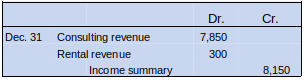
\includegraphics[width=0.6\columnwidth]{images/c4/closing_revenue.png}
		\end{figure}
		\item \textbf{Close all expense accounts to the income summary.} This 
		will zero out all our expense accounts.
		\begin{figure}[ht]
			\centering
			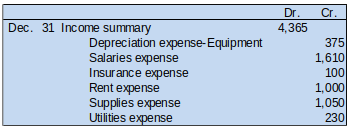
\includegraphics[width=0.60\columnwidth]{images/c4/close_expenses.png}
		\end{figure}
		\item \textbf{Close the income summary} which contains net profit, 
		to 
		retained 
		earnings. This process zeroes out the income summary.
		\begin{figure}[ht]
			\centering
			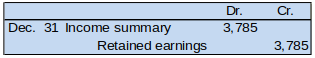
\includegraphics[width=0.60\columnwidth]{images/c4/close_income_summary.png}
		\end{figure}
		\item \textbf{Move the dividends to retained earnings.} This will cause 
		the dividends account to have a zero balance.
		\begin{figure}[ht]
			\centering
			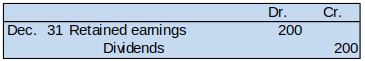
\includegraphics[width=0.60\columnwidth]{images/c4/close_dividends.png}
		\end{figure}
	\end{enumerate}
	
	\begin{figure}[ht]
		\centering
		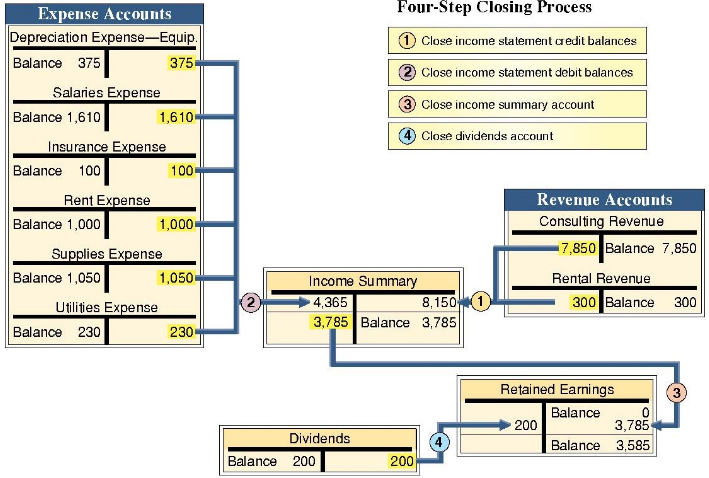
\includegraphics[width=1\columnwidth]{images/c4/closing_summary.png}
		\caption{Closing Summary}
	\end{figure}
	
	\subsubsection{Post-Closing Trial Balance}
	
	After all four of our closing entries have been made, we prepare a 
	post-closing trial balance. This trial balance should show only permanent 
	accounts, that is assets, liabilities, and the equity account. All the 
	revenues, expenses, and dividends have been reduced to zero balances. The 
	total debits and credits in this trial balance must be equal.
	
	\begin{figure}[ht]
		\centering
		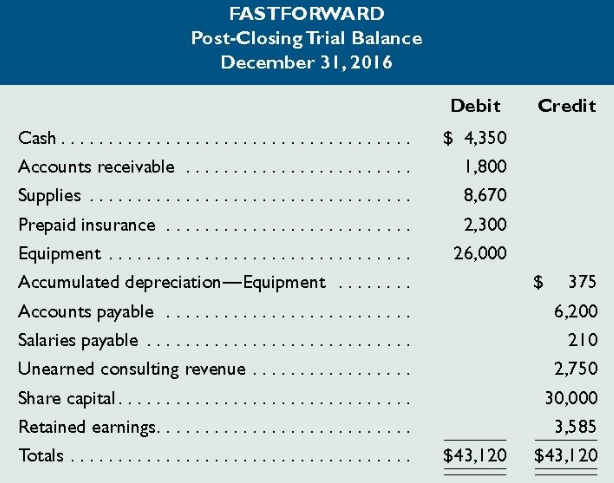
\includegraphics[width=0.9\columnwidth]{images/c4/post_closing_trial_balance.png}
		\caption{\textbf{Post-Closing Trial Balance.} Notice that the retained 
		earnings account has been updated to include net profit and dividends.}
	\end{figure}
	
	
\end{document}